\chapter{Les Théories Basses Fidélités}
\label{ch:Ch1}

%%%%%%%%%%%%%%%%%%%%%%%%%%%%%%%%%%%% SECTION 1
\section{La théorie de la ligne portante (continue)} 
\label{sec:Ch1.1}

%%%%%%%%%%%%% SUBSECTION 1.1
\subsection{La théorie} 
\label{subsec:Ch1.1.1}

\begin{figure}[H]
    \centering
    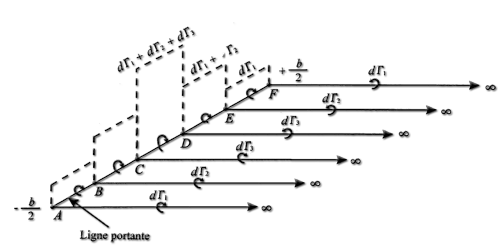
\includegraphics[width=0.7\textwidth]{Pics/01 - Basses Fidélités/Ligne portante.png}  
    \caption{Vortex en fer à cheval de la ligne portante}
    \label{fig:llt fer à cheval}
\end{figure}

La théorie des lignes portantes utilise la conception de circulation et le théorème de Kutta-Jukowski qui affirme que :

\begin{center}
    \begin{equation}
        L(y) = \rho v \Gamma(y)
        \label{eq:Cl_breukels}
    \end{equation}
\end{center}

Aussi, la circulation élémentaire en un point M $\delta\Gamma(M) $ induit une vitesse en P $d\omega(P) $ selon : 

\begin{center}
    \begin{equation}
        d\omega(M) = \frac{\delta\Gamma(P) \times \overrightarrow{PM}}{4\pi ||\overrightarrow{PM}||^3}
        \label{eq:v induite}
    \end{equation}
\end{center}

Ce qui le long de la ligne portante, axe des y, donne : 

\begin{center}
    \begin{equation}
        dv_i(y_0) = \frac{\delta\Gamma(y)}{4\pi (y-y_0)^2}
        \label{eq:v induite 1d}
    \end{equation}
\end{center}

En intégrant l'équation \ref{eq:v induite 1d} selon y, on remonte ainsi à l'angle induit en $y_0$ : 
\begin{center}
    \begin{equation}
        \alpha_i(y_0) = \frac{v_i(y_0)}{v_{\infty}}
        \label{eq:angle induit}
    \end{equation}
\end{center}

\begin{figure}[H]
    \centering
    % Première image
    \begin{subfigure}[b]{0.45\textwidth}
        \centering
        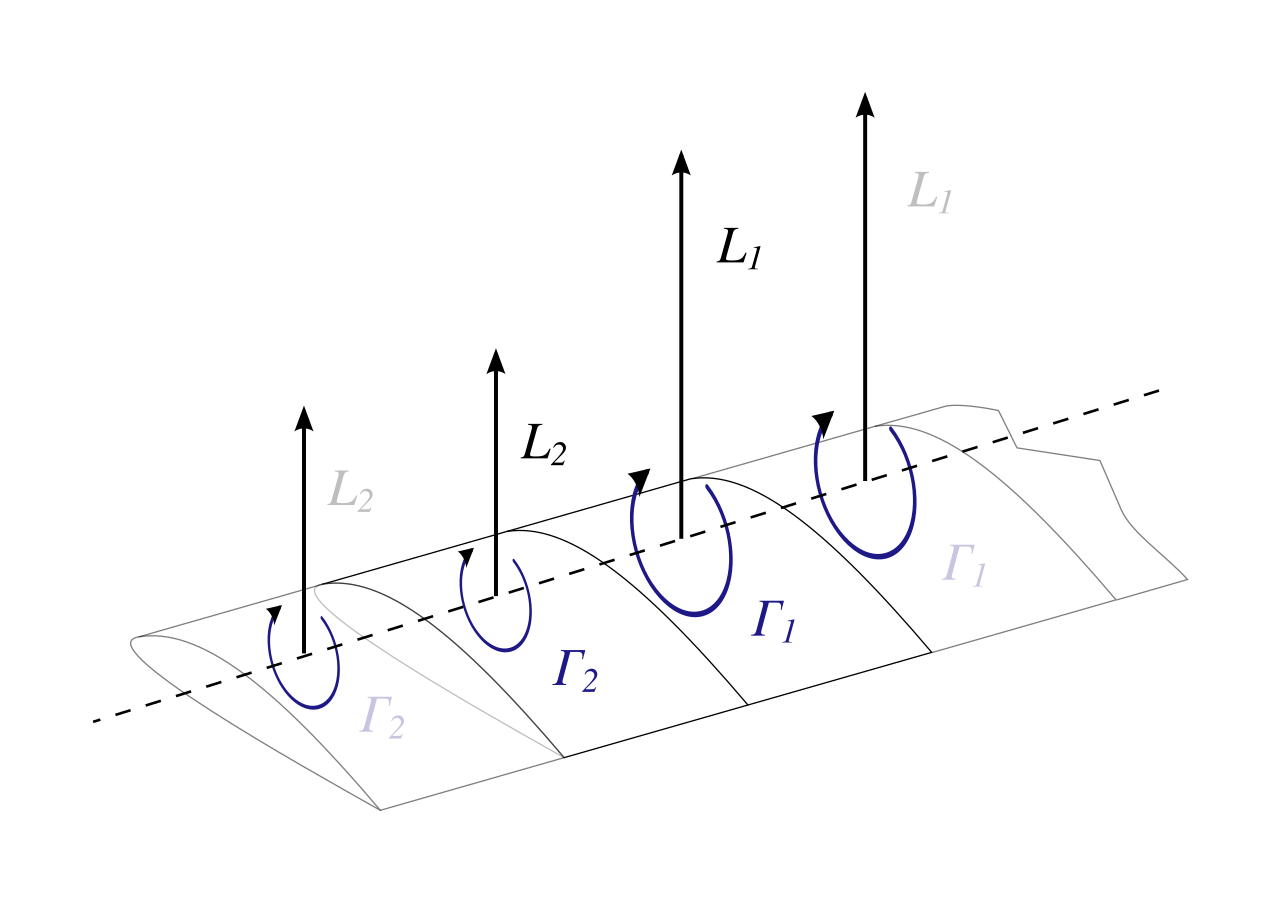
\includegraphics[width=\textwidth]{Pics/01 - Basses Fidélités/LLT KJ.png}
        \caption{Lien Portance - Circulation}
        \label{fig:LLT KJ}
    \end{subfigure}
    \hfill
    % Deuxième image
    \begin{subfigure}[b]{0.45\textwidth}
        \centering
        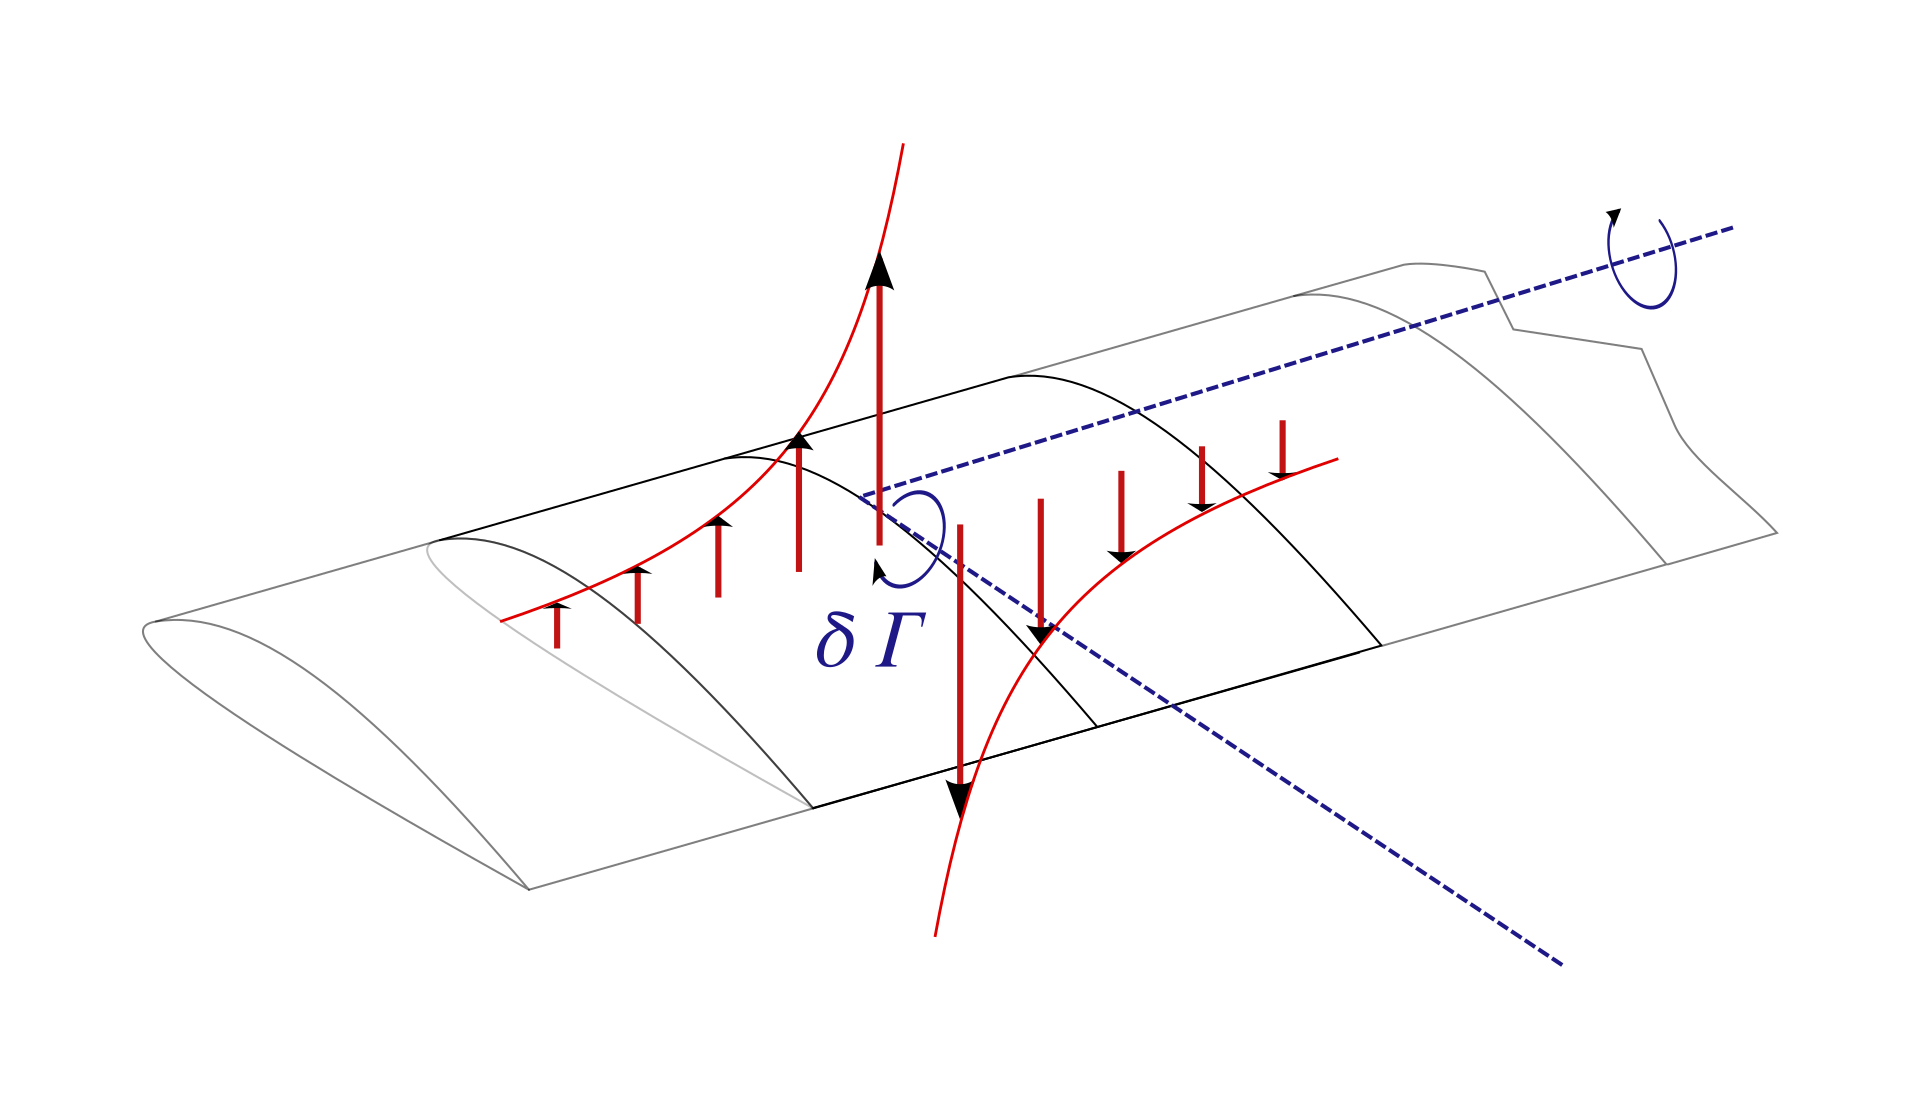
\includegraphics[width=\textwidth]{Pics/01 - Basses Fidélités/LLT vortex.png}
        \caption{Lien Circulation - Vitesse induite}
        \label{fig:LLT vortex}
    \end{subfigure}
\end{figure}

Ainsi, on a :

\begin{equation}
    L_{total} = \rho v_{\infty} \int_{-\frac{b}{2}}^{\frac{b}{2}} \Gamma(y) dy
\end{equation}

et, avec $v_{\infty} sin(\alpha_i(y)) = v_i(y)$ car $tan(\alpha_i(y)) = \frac{v_i(y)}{v_{\infty}}$, on a :
\begin{equation}
    D_{i,total} = \rho \int_{-\frac{b}{2}}^{\frac{b}{2}} v_{i}(y)\Gamma(y) dy
\end{equation}

%%%%%%%%%%%%% SUBSECTION 1.2
\subsection{La résolution} 
\label{subsec:Ch1.1.2}

Pour résoudre un problème avec la LLT on utilise la méthode suivante : 

\begin{figure}[H]
    \centering
    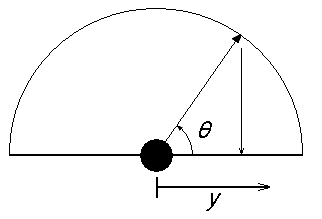
\includegraphics[width=0.5\textwidth]{Pics/01 - Basses Fidélités/Prandtl-lifting-line-coordinate-change.png}  
    \caption{Changement de coordonées}
    \label{fig:llt fchange coord}
\end{figure}

On pose $y = -\frac{b}{2}cos(\theta)$ et $\Gamma(\theta) = 2bv_{\infty} \sum_{n \in \mathbb{N}}^{} A_n sin(n\theta)$, on a alors :

\begin{equation}
    \begin{split}
        \frac{\rho v \Gamma}{P_{dynamique} S} = \frac{L}{P_{dynamique} S} = C_L = C_{L,\alpha,3D}(\alpha - \alpha_{0,3D} - \Delta\alpha_{vrillage} - \alpha_{induit}) \\
        \Leftrightarrow 2b\sum_{n \geq 1}^{} A_n sin(n\theta) = \pi (\alpha - \alpha_{0,3D} - \Delta\alpha_{vrillage} - \sum_{n \geq 1}^{}n A_n \frac{sin(n\theta)}{sin(\theta)})c(y)
    \end{split}
    \label{eq: LLT}
\end{equation}

On remarque dans l'équation \ref{eq: LLT} que la LLT utilise donc la théorie 2D des profils minces ($C_L = C_{L, \alpha, 2D}(\alpha - \alpha_{0,2D})$) avec une formule simple de passage des coefficients 2D à 3D (dépend de l'allongement de l'aile)

Finalement, \textbf{en faisant l'hypothèse de la théorie 2D des profils minces, et à partir de la loi de corde $c(y)$ uniquement}, on peut calculer la circulation 3D d'une aile $\Gamma(y)$, sa Portance $L$, sa trainée induite $D_i$, et sa vitesse induite $v_i(y)$

%%%%%%%%%%%%%%%%%%%%%%%%%%%%%%%%%%%% SECTION 2
\section{La Ligne Portante - Implémentation numérique (discret)} 
\label{sec:Ch1.2}

On s'intéresse maintenant à l'application de cette théorie aux simulations numériques basses fidélités. En outre, on s'intéresse à son implémentation. 

%%%%%%%%%%%%% SUBSECTION 2.1
\subsection{LLT - Lifting Line Theory} 
\label{subsec:Ch1.2.1}

On discrétise l'aile par \textbf{panneaux le long de l'envergure}. Chaque panneaux i est associé à une cirulation $\Gamma_i$, une portance $L_i$, et une trainée $D_i$ et une vitesse induite $v_{ind}$ (orthogonale à $v_{\infty}$) à $\frac{1}{4}$ de la corde.

\begin{figure}[H]
    \centering
    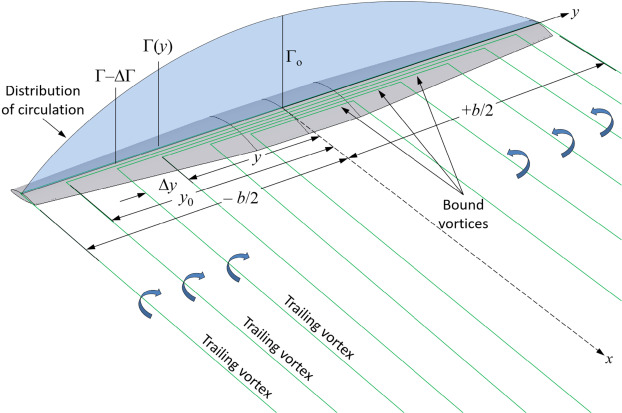
\includegraphics[width=0.9\textwidth]{Pics/01 - Basses Fidélités/LLT schéma.jpg}
    \caption{Représentation du modèle de ligne portante constitué de tourbillons en fer à cheval}
    \label{fig: vortex vsm}
\end{figure}

\textbf{La Lifting Line Theory considère que le point d'application des efforts aéro (i.e. là où passe la ligne portante), et le "collocation point" où s'applique la vitesse induite orthogonale à la vitesse à l'infinie (i.e. là où l'écoulement est dévié de l'angle induit $\alpha_{ind} = \frac{v_{inf}}{V_{\infty}}$) sont tous deux à 1/4 de la corde. C'est la principale différence avec la VSM}

L'équation \ref{eq:v induite} permet d'écrire en le panneaux i:
\begin{equation}
    v_i = \sum_{panneaux j}^{} v_{j,i} = \sum_{panneaux j}^{} b_{j,i} \Gamma_j
    \label{eq: v induite j}
\end{equation}
avec $v_i$ la vitesse induite en i, $v_{j,i}$ la vitesse induite en i par le panneaux j, et $b_{j,i}$ un coefficient d'influence (géométrique) du panneaux j sur le panneaux i. Donc 

\begin{equation}
    V_{ind} = AIC .\Gamma
    \label{eq: v induite j matrice}
\end{equation}

avec $V \in M_n(\mathbb{R})$, $\Gamma \in M_n(\mathbb{R})$, et $AIC \in M_{n,n}(\mathbb{R})$ la matrice d'influence

De plus, en combiant \ref{eq: LLT} et \ref{eq: v induite j matrice}, en sachant que $\alpha_i = \frac{v_i}{v_{\infty}}$, on obtient une équation de la forme : 

\begin{equation}
    \frac{1}{v_{\infty}}\Gamma = \pi c (\alpha-\alpha_{0,3D} - \Delta\alpha_v - \frac{1}{v_{\infty}} AIC.\Gamma)
    \label{eq: LLT gamma}
\end{equation}
avec $c \in M_{1,n}(\mathbb{R})$ la matrice dont la colonne j correspond à la valeur de la corde en le $j^{ème}$ panneaux.

Finalement, on peut écrire \ref{eq: LLT gamma} sous la forme :

\begin{equation}
    A \Gamma = B
    \label{eq: LLT gamma 2 }
\end{equation}

Ainsi on peut calculer $\Gamma$, en déduire les vitesses induites $V_{ind}$, calculer la répartition des forces de portance et de trainée $L_i = \rho v_{\infty} \Gamma_i$ et $D_i = \rho v_i \Gamma_i$, et sommer pour obtenir les forces de portance et de trainée.

Finalement, en faisant \textbf{l’hypothèse de la théorie 2D des profils minces ($C_{L, \alpha, 2D}$ et $\alpha_{0, 2D}$)}, et à partir de la \textbf{loi de corde uniquement (matrices c et AIC)}, on peut calculer la circulation 3D d’une aile $\Gamma$, sa Portance $L$, sa trainée induite $D_i$, et sa vitesse induite $v_i$. \\
A noter qu'il existe une formule simple qui permet de calculer $C_{L, \alpha, 3D}$ et $\alpha_{0, 3D}$ à partir de $C_{L, \alpha, 2D}$ et $\alpha_{0, 2D}$ et de l'allongement de l'aile.

%%%%%%%%%%%%% SUBSECTION 2.2
\subsection{LP3DNLI (Théo Simonet - EAE)} 
\label{subsec:Ch1.2.2}

%%%%%%%%%%%%% SUBSECTION 2.3
\subsection{VSM - Vortex Step Method} 
\label{subsec:Ch1.2.3}

\textbf{Hypothèses} \\
\begin{itemize}
    \item L'écoulement peut être divisé en deux régions : la région interne et la région externe. D'une part, l'écoulement dans la région interne représente les propriétés du profil aérodynamique, qui peuvent être obtenues par une variété de méthodes. D'autre part, l'écoulement en dehors de la région du profil est sans viscosité, irrotationnel et incompressible, afin d'obtenir une solution d'écoulement potentiel.
    \item Le théorème de Kutta–Joukowski est satisfait dans chaque section de l'aile, reliant les régions interne et externe.
    \item L'écoulement est quasi-stationnaire, ce qui signifie que chaque condition d'écoulement peut être résolue uniquement dans le domaine spatial.
    \item Le vortex de départ est situé très en aval et son influence peut être négligée.
    \item HYPOTHÈSE DU SILLAGE FIGÉ.
\end{itemize}

\textbf{La VSM considère que le point d'application des efforts aéro (i.e. là où passe la ligne portante) est à 1/4 de la corde, et que le "collocation point" où s'applique la vitesse induite orthogonale à la vitesse à l'infinie (i.e. là où l'écoulement est dévié de l'angle induit $\alpha_{ind} = \frac{v_{inf}}{V_{\infty}}$) est à 3/4 de la corde. C'est la principale différence avec la LLT}

\textbf{Système de vorticity}
\begin{figure}[H]
    \centering
    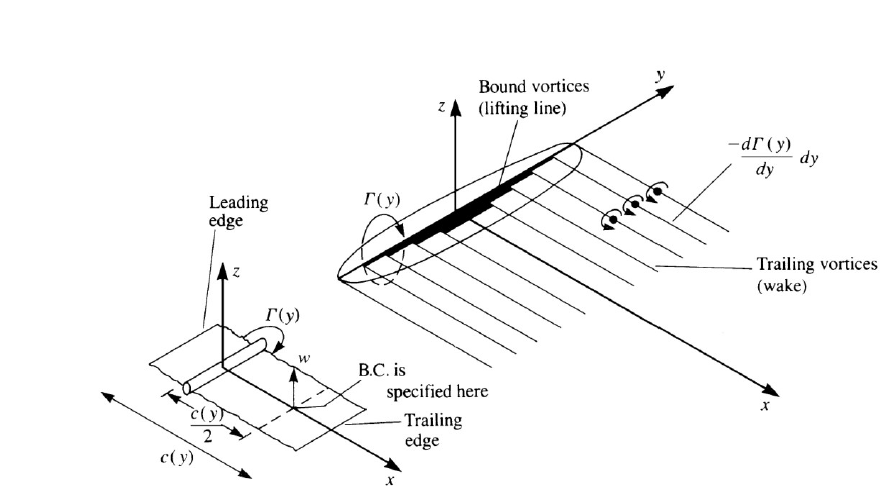
\includegraphics[width=0.7\textwidth]{Pics/01 - Basses Fidélités/vortex VSM.png}
    \caption{Représentation du modèle de ligne portante constitué de tourbillons en fer à cheval}
    \label{fig: vortex vsm}
\end{figure}


Dans la théorie classique de la ligne portante de Prandtl, la ligne portante est supposée être droite, et les tourbillons traînants sont uniquement responsables de l'induction du vent induit qui modifie les angles d'attaque locaux. En revanche, dans un cas plus général, où la ligne portante n'est pas droite, comme dans le cas du VSM actuellement étudié, l'ensemble du système de vorticité joue un rôle dans le changement de l'angle d'attaque sectionnel.\\

\begin{figure}[H]
    \centering
    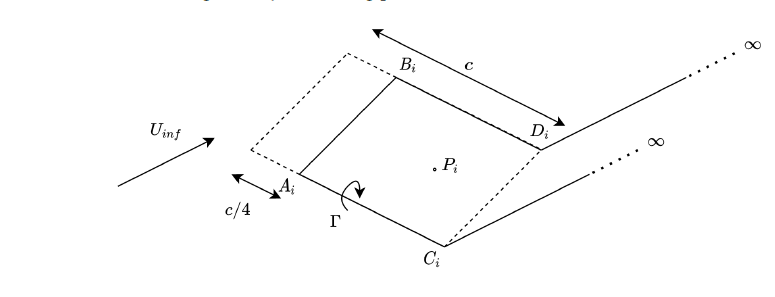
\includegraphics[width=0.7\textwidth]{Pics/01 - Basses Fidélités/Panneaux VSM.png}
    \caption{Représentation de la géométrie d'un vortex en fer à cheval}
    \label{fig:panneau vsm}
\end{figure}

\textbf{Les vitesses induites des panneaux J sur les points de control i}

Ces vitesses induites sont compliquées à exprimer selon si on se situe sur un panneaux ou un filament infinie. La formule générale, issue de la théorie de la ligne portante, est la suivante : 
\begin{equation}
    dw = \frac{\Gamma}{4 \pi} \frac{\overrightarrow{dl} \times \overrightarrow{r}}{|\overrightarrow{r}|^3}
    \label{eq: LLT vi}
\end{equation}

\textbf{Matrice d'influence AIC}

Ainsi, grâce à \ref{eq: LLT vi} on lie vitesse induite en un point de control i par l'ensemble des circulations $\Gamma$ des panneaux j via des matrices d'influences : 
\begin{equation}
    u = AIC_u \Gamma
    \label{eq:gamma}
\end{equation}

\textbf{Calcul de la circulation}
\begin{equation}
    \rho |U_{\infty} \Gamma_j| - \frac{1}{2} \rho |U_{rel} z_{airf}|^2 c C_l(\alpha_{EFF_j}) = 0
    \label{eq:gamma_new}
\end{equation}

\textbf{Résolution par itération à convergence}\\
On part d'une circulation $\Gamma$ initiale, on en déduit la vitesse induite (eq. \ref{eq:gamma}), on calcul l'angle induit ($\alpha_{ind} = \frac{v_{ind}}{v_{\infty}}$) ($\alpha_{tot} = \alpha + \alpha_{ind}$), on calcul $C_l(\alpha)$ (ici, avec le code de Ocaryon, on utilise la formule de régression de Breukels), puis on calcul à nouveau $\Gamma$ grâce à l'équation \ref{eq:gamma_new}. On itère le procédé jusqu'à convergence...\\

\textbf{En conclusion}\\
\textbf{la VSM utilise la loi de corde de l'aile (relation \ref{eq:gamma}) \& la polaire 2D par regression de Breukels (i.e. CFD 2D sur kites à boudin), le tout lié par les relations de la théorie de la ligne portante (\ref{eq: LLT vi}, \ref{eq:gamma} \ref{eq:gamma_new})}\\

\textbf{A noter que cette méthode de résolution utilise les mêmes théories/calculs que la LLT mais en by-passant l'inversion de matrice par des itérations à convergence sur le calcul de la loi/répartition de circulation $\Gamma$}\\

%%%%%%%%%%%%%%%%%%%%%%%%%%%%%%%%%%%% SECTION 3
\section{La Surface Portante - Implémentation numérique (discret)} 
\label{sec:Ch1.3}

%%%%%%%%%%%%% SUBSECTION 2.3
\subsection{VLM - Vortex Latex Method} 
\label{subsec:Ch1.3.1}

Les hypothèses suivantes sont formulées concernant le problème dans la méthode du réseau tourbillonnaire (vortex lattice method) :\\
\begin{itemize}
    \item Le champ d'écoulement est incompressible, non visqueux et irrotationnel. Cependant, un écoulement compressible subsonique avec de faibles perturbations peut être modélisé si la transformation générale tridimensionnelle de Prandtl-Glauert est intégrée dans la méthode.
    \item Les surfaces portantes sont minces. L'influence de l'épaisseur sur les forces aérodynamiques est négligée. C'est la \textbf{théorie des surfaces minces}
    \item L'angle d'incidence (angle d'attaque) et l'angle de dérapage sont tous deux petits, ce qui permet l'utilisation de l'approximation des petits angles.
\end{itemize}

\textbf{On discrétise cette fois une aile en plein de panneaux le long de l'envergure et de la corde. Pour ce faire, on représent l'aile par sa loi de cambrure moyenne (pour que cela fasse une surface en 3D). Comme avec a LLT on considère qu'en chaque panneaux s'appliquent une portance via une circulation (vortex en fer à cheval) à $\frac{1}{4}$ de la corde et un point de collocation à $\frac{1}{4}$ de la corde}

\begin{figure}[H]
    \centering
    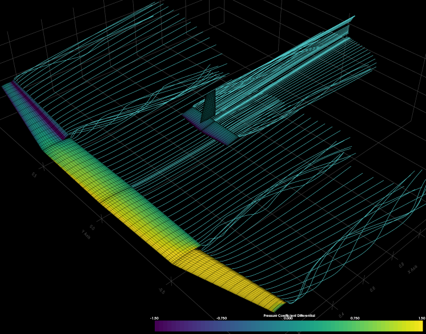
\includegraphics[width=0.7\textwidth]{Pics/01 - Basses Fidélités/vlm.png}
    \caption{Illustration de la VLM avec ses panneaux de discrétisation et les lignes de vortex en fer à cheval dans le sillage de l'avion}
    \label{fig:vlm}
\end{figure}

On applique en chaque point de collocation ($\frac{1}{4}$ de la corde) la \textbf{condition aux limites de Neumann} qui impose que la vitesse ($\overrightarrow{v_i} = \overrightarrow{v_{\infty}} + \overrightarrow{v_{induite,i}}$) soit orthogonale au panneaux (\textbf{condition d'imperméabilité}) :
\begin{equation}
    \overrightarrow{v_i}.\overrightarrow{n_i} = (\overrightarrow{v_{\infty}} + \sum_{j =1}^{N}\overrightarrow{v_{j,i}}).\overrightarrow{n_i} = (\overrightarrow{v_{\infty}} + \sum_{j =1}^{N}w_{j,i}\overrightarrow{\Gamma_j}).\overrightarrow{n_i} = 0
    \label{eq: Neumann boundary}
\end{equation}

On remarque que la vitesse induite par un panneaux j sur un panneaux i $\overrightarrow{v_{j,i}}$ est liée à la circulation du panneaux j $\Gamma_j$ par un coefficient d'influence $w_{j,i}$ \textbf{exactement comme pour la théorie de la ligne portante}, ce qui ici s'appelle \textbf{la théorie de la surface portante}.

Finalement, en posant $A = (a_{i,j})_{0 \leq (i,j) \leq N}$ la matrice d'influence, $B = (b_{j})_{0 \leq j \leq N}$, $a_{i,j} = \frac{w_{i,j}\overrightarrow{\Gamma_j}.\overrightarrow{n_i}}{||\overrightarrow{\Gamma_j}||}$, et $b_{i} = \overrightarrow{v_{\infty}}.\overrightarrow{n_i}$, on résoud à nouveau un système (inversion de matrice ou itération sur la loi de $\Gamma$ jusqu'à convergence) :

\begin{equation}
    A.\Gamma = B
    \label{eq : vlm gamma}
\end{equation}

De là, on peut calculer la résultante aéro de chaque panneaux (la condition de Neumann impose une vitesse tangente au panneaux donc cette force est suivant $\overrightarrow{n_i}$), puis la force totale, le moment total, la trainée induite (par l'angle induit par les vortex en fer à cheval), et la portance: 

\begin{equation}
    \begin{split}
        \overrightarrow{F_i} = \rho \Gamma_i(v_{\infty} + v_{i,ind})l_i \overrightarrow{n_i} \\
        \overrightarrow{F} = \sum_{i=0}^{N}\overrightarrow{F_i} \\
        \overrightarrow{M} = \sum_{i=0}^{N}\overrightarrow{F_i} \overrightarrow{r_i} \\
        D_{ind} = \overrightarrow{F_i}.\overrightarrow{e_x} \overrightarrow{e_x} \\
        L = \overrightarrow{F_i}.\overrightarrow{e_z} \overrightarrow{e_z}
    \end{split}
    \label{eq : vlm resultats}
\end{equation}
Avec $l_i$ la longueur transverse du panneaux (selon l'envergure).

\textbf{Remarque : là où VSM et LLT considèrent le point de collocation comme étant là où la vitesse induite est orthogonale à la vitesse à l'infinie($\alpha_i = \frac{v_i}{v_{\infty}}$), la VLM considère son point de collocation comme l'endroit où s'applique la condition d'imperméabilité ($(\overrightarrow{v_{\infty}} + \overrightarrow{v_{ind}}).\overrightarrow{n} = 0$)}\\

\textbf{Remarque bis : la condition de non pénétration est ce qui permet d'obtenir les résultat de la théorie 2D des profils minces ($C_L = C_{L, \alpha}(\alpha - \alpha_{0,2D}) = 2\pi (\alpha - \alpha_{0,2D})$). Pour ce faire il faut rajouter la condition de Kutta-Joukowski qui permet de fermer le système d'équation (N équations à N inconnues) et se traduit par $\frac{d\Gamma}{dt} = 0$ et donc $\Gamma_N = \Gamma_0$; qui sont les $\Gamma$ du BF sur l'intrados et l'extrados (car on discrétise le profil par N panneaux du BF au BF en passant par le BA, de l'extrados à l'intrados)}\\

Finalement, \textbf{en faisant l'hypothèse de la théorie 2D des profils minces sur chaque panneaux (via condition de non pénétration), à partir de la loi de corde $c(y)$ (matrice d'influence AIC notée A), et à partir de la loi de cambrure moyenne (discrétisation le long de la corde)}, on peut calculer la circulation 3D d'une aile $\Gamma_i$, sa Portance $L$, sa trainée induite $D_{ind}$, et sa vitesse induite $v_{i, ind}$. On ne parle plus de ligne portante mais plutôt de \textbf{surface portante} car désormais chaque panneaux à un vortex élémentaire $\delta\Gamma_i$ au $\frac{1}{4}$ de la corde, repartit sur toute l'aile (envergure + corde), qui génère sa portance élémentaire $\delta L_i$.


%%%%%%%%%%%%%%%%%%%%%%%%%%%%%%%%%%%% SECTION 4
\section{Comparaison} 
\label{sec:Ch1.4}

\begin{table}[h!]
    \centering
    \begin{tabular}{|p{2.8cm}|p{1.6cm}|p{2cm}|p{3cm}|p{2cm}|}
        \hline
        & \textbf{LLT} & \textbf{VSM} & \textbf{VLM} & \textbf{LP3DNLI} \\ \hline
        \textbf{Théorie 3D} & Ligne Portante & Ligne Portante & Surface Portante & Ligne Portante\\ \hline
        \textbf{Discrétisation} & Envergure & Envergure & Envergure ET corde selon la loi de cambrure moyenne & Envergure \\ \hline
        \textbf{Théorie 2D} & Théorie profils minces & Regression Breukels (CFD 2D) OU n'importes quels données de polaires 2D & Théorie profils minces par panneaux + matrice d'influence & Théorie profils minces OU n'importes quels données de polaires 2D \\ \hline
        \textbf{Déclinaison LLT continue en discret} & Matrice d'influence & Matrice d'influence & Matrice d'influence & Matrice d'influence\\ \hline
        \textbf{Représentation d'une section} & Profil mince (problème portant (+ problème épais ?)) & Airfoil & Panneaux discret (eux-mêmes profils minces (plaque plane donc problème portant sans cambrure)) & Profil mince (problème portant (+ problème épais ?)) \\ \hline
        \textbf{Passage 2D à 3D} & Loi de corde et matrice d'influence AIC & Loi de corde et matrice d'influence AIC & Loi de corde et matrice d'influence AIC & Loi de corde et matrice d'influence AIC\\ \hline
        \textbf{Prise en compte de la cambrure via} & calcul 2D & calcul 2D & discrétisation selon la loi de cambrure moyenne & calcul 2D\\ \hline
        \textbf{Point d'application des efforts aéro} & 1/4 corde & 1/4 corde & 1/4 corde & 1/4 corde\\ \hline
        \textbf{Collocation Point} & 1/4 corde & 3/4 corde & 1/4 corde & 1/4 cord \\ \hline
        \textbf{Prise en compte du décrochage} & Non & possible avec CFD 2D (Breukels) & Non & Oui (modèle de stall 3D) + possible avec CFD 2D (Breukels) \\ \hline
    \end{tabular}
    \caption{Tableau de comparaison des théories}
    \label{tab:comparaison}
\end{table}